Веб-приложение состоит из двух основных частей: back-end и front-end. Back-end -- это сам веб-сервер,
который осуществляет обработку запросов пользователей, получение и обработку данных.
Front-end -- это пользовательский интерфейс, визуализирующий полученные от back-end данные в понятный вид.
С помощью этого интерфейса пользователь способен не только получать, но и передавать данные на back-end.

Back-end составляющая сервиса реализована на языке Python 3, с использованием библиотек: Flask~---
обрабатывает HTTP запросы от пользователей, pandas~--- обработка и хранение данных; sklearn~--- модели TFIDF, KMeans, SVM;
pymystem3~--- лемматизация.

Структура приложения показана на рис. \ref{server_struct}.

\begin{figure}[h]
    \centering
    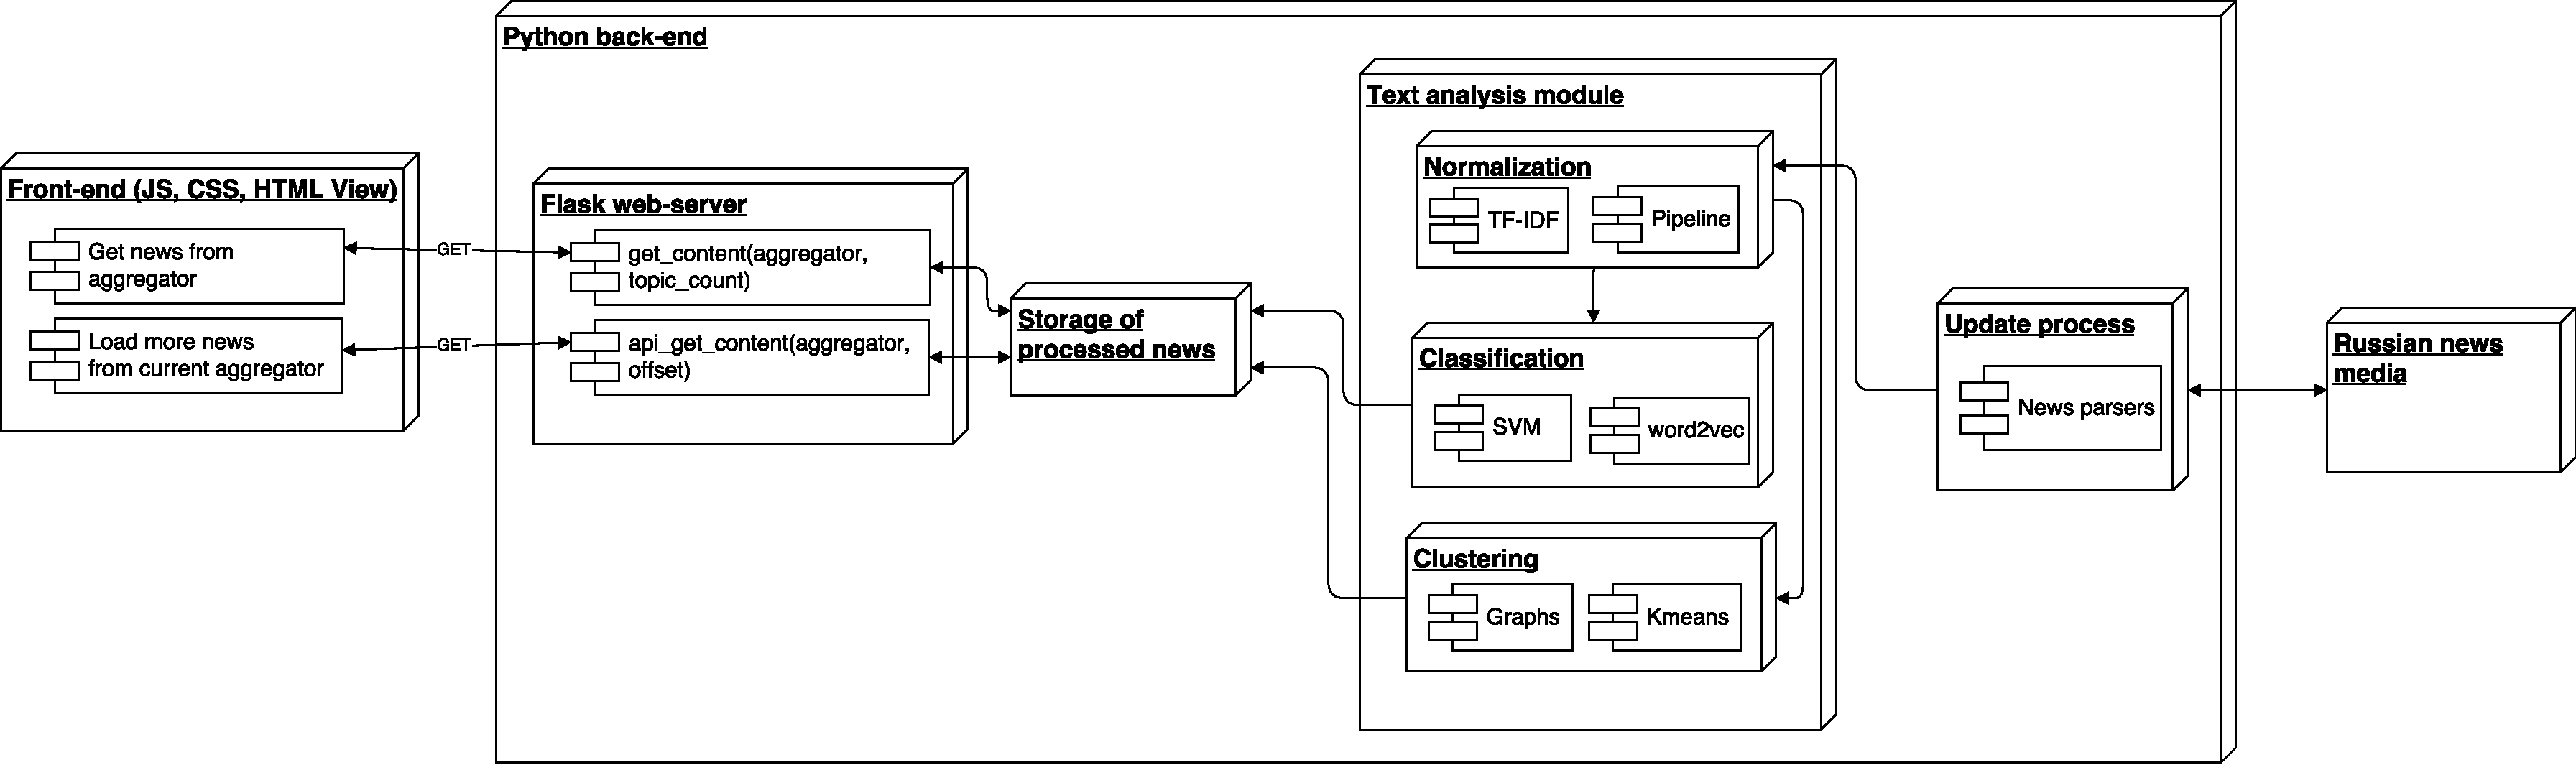
\includegraphics[width=1\textwidth]{server_infrastructure.pdf}
    \caption{Структура сервера}
    \label{server_struct}
\end{figure}

Back-end разделён на несколько модулей: Flask web-сервер, модуль парсеров новостей, которые
с помощью параллельных процессов извлекают данные с сайтов СМИ, модуль анализа данных.

При запуске сервера происходит получение новостей за последние 12 часов и их обработка.
После этого запускается отдельный процесс, отвечающий за актуальность данных: каждую минуту он
проверяет наличие новых статей, и, если такие есть, отправляет их на обработку. При запросе от Front-end, сервер
обращается к уже обработанным данным, хранящимся в кэше.

% \subsection{Back-end часть}
% \subsection{Front-end часть}